\documentclass{article}
\usepackage{tikz}
\usepackage{bm}
\usetikzlibrary{positioning, arrows.meta, shapes.geometric, fit, calc, decorations.pathreplacing}
\begin{document}
\begin{figure}[h]
\centering
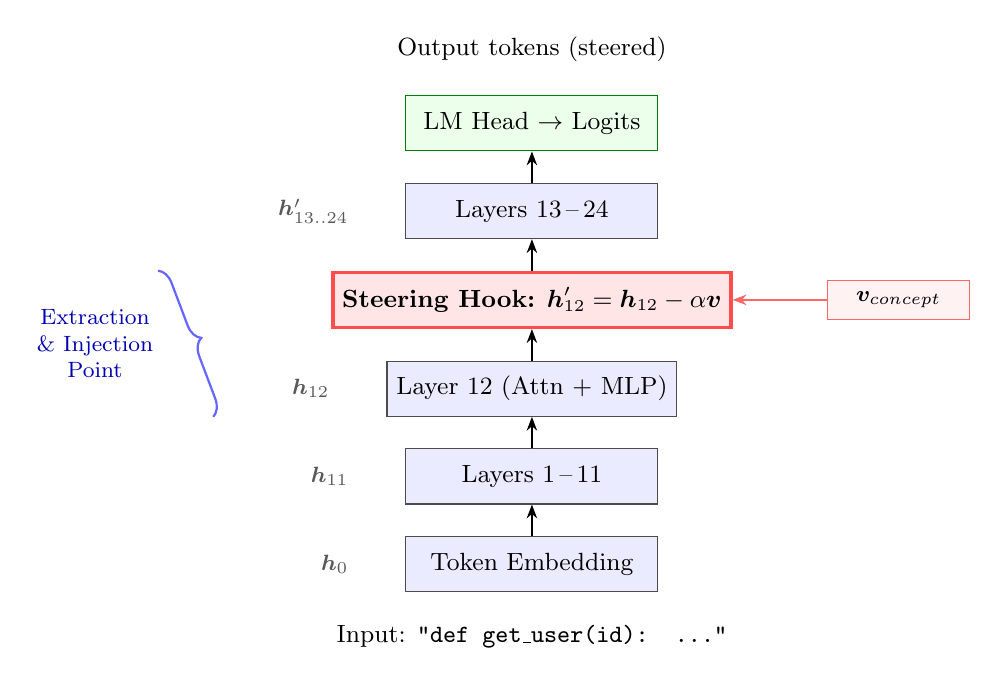
\begin{tikzpicture}[
    block/.style={rectangle, draw=black!70, fill=blue!8, minimum width=3.2cm, minimum height=0.7cm, font=\small},
    hookblock/.style={rectangle, draw=red!70, fill=red!10, minimum width=3.2cm, minimum height=0.7cm, font=\small, line width=1.2pt},
    arrow/.style={-{Stealth[length=5pt]}, thick},
    label/.style={font=\footnotesize\itshape, text=gray!70!black},
]
% Embedding
\node[block] (emb) {Token Embedding};
\node[label, left=0.6cm of emb] {$\bm{h}_0$};

% Layers 1-11
\node[block, above=0.4cm of emb] (l1) {Layers 1\,--\,11};
\node[label, left=0.6cm of l1] {$\bm{h}_{11}$};

% Layer 12
\node[block, above=0.4cm of l1] (l12) {Layer 12 (Attn + MLP)};
\node[label, left=0.6cm of l12] {$\bm{h}_{12}$};

% Steering Hook
\node[hookblock, above=0.4cm of l12] (hook) {\textbf{Steering Hook:} $\bm{h}'_{12} = \bm{h}_{12} - \alpha\bm{v}$};

% Concept vector annotation
\node[rectangle, draw=red!60, fill=red!5, minimum width=1.8cm, minimum height=0.5cm, font=\footnotesize, right=1.2cm of hook] (vec) {$\bm{v}_{\text{concept}}$};
\draw[arrow, red!60] (vec) -- (hook);

% Layers 13-24
\node[block, above=0.4cm of hook] (l13) {Layers 13\,--\,24};
\node[label, left=0.6cm of l13] {$\bm{h}'_{13..24}$};

% LM Head
\node[block, above=0.4cm of l13, fill=green!8, draw=green!50!black] (head) {LM Head $\rightarrow$ Logits};

% Arrows
\draw[arrow] (emb) -- (l1);
\draw[arrow] (l1) -- (l12);
\draw[arrow] (l12) -- (hook);
\draw[arrow] (hook) -- (l13);
\draw[arrow] (l13) -- (head);

% Input/Output labels
\node[below=0.3cm of emb, font=\small] {Input: \texttt{"def get\_user(id): ..."}};
\node[above=0.3cm of head, font=\small] {Output tokens (steered)};

% Brace for extraction point
\draw[decorate, decoration={brace, amplitude=6pt, mirror}, thick, blue!60] ([xshift=-2.2cm]l12.south west) -- ([xshift=-2.2cm]hook.north west) node[midway, left=8pt, font=\footnotesize, text=blue!70!black, align=center] {Extraction\\\& Injection\\Point};
\end{tikzpicture}
\end{figure}
\end{document}
